\section{Experimentos}
Comparamos nossas implementações com o
\gzip\footnote{\url{http://www.gzip.org/}},
grep\footnote{\url{https://www.gnu.org/software/grep/}} e com o
codesearch\footnote{\url{https://github.com/google/codesearch}}.
Realizamos experimentos para responder às seguintes perguntas:
\begin{enumerate}
\item \rqone
\item \rqtwo
\item \rqthree
\end{enumerate}

Foram implementados scripts em BASH para controlar os experimentos e fazer
medições, gerando arquivos .raw de saída contendo resultados. Foram também
implementados scripts em R que desenham gráficos de acordo com os arquivos .raw
gerados pelos scripts BASH.


Todos os experimentos foram realizados em uma máquina com processador Intel Core
i5 2.6Ghz e 8Gb de RAM. Cada medição de tempo nos experimentos foi realizada 10
vezes, e somente a média foi considerada e reportada nos resultados.
Todos os scripts e resultados estão disponíveis no diretório {\it experiments}.

\subsection{\rqone}
Nós comparamos a nossa implementação do \lz com o \gzip em dois aspectos: Tempo
e taxa de compressão.
Para realizar essa comparação, primeiramente nós dividimos um arquivo\footnote{
\url{http://pizzachili.dcc.uchile.cl/texts/nlang/english.1024MB.gz}}
que contém 1GB de texto em inglês em arquivos de
tamanhos distintos: 100KB, 200KB, 300KB, 700KB, 1MB, 2MB, 3MB, 5MB, 50MB, 100MB,
200MB, 300MB e 500MB. Cada arquivo desse contém os primeiros n bytes do
arquivo original, onde n é o tamanho do arquivo. Fizemos medições em relação ao
tempo e à taxa de compressão para cada operação de compressão e descompressão
levando em conta os algoritmos \lz e gzip.

Separadamente, repetimos também o mesmo experimento acima mas
usando como entrada um arquivo\footnote{\url{http://pizzachili.dcc.uchile.cl/texts/protein/proteins.200MB.gz}}
de 200MB contendo sequências de proteinas. Esse arquivo também foi divido
em arquivos de tamanhos distintos: 100KB, 200KB, 300KB, 700KB, 1MB, 2MB, 3MB, 5MB,
50MB, 100MB, 200MB.

\subsubsection{Tempo}


\begin{figure}
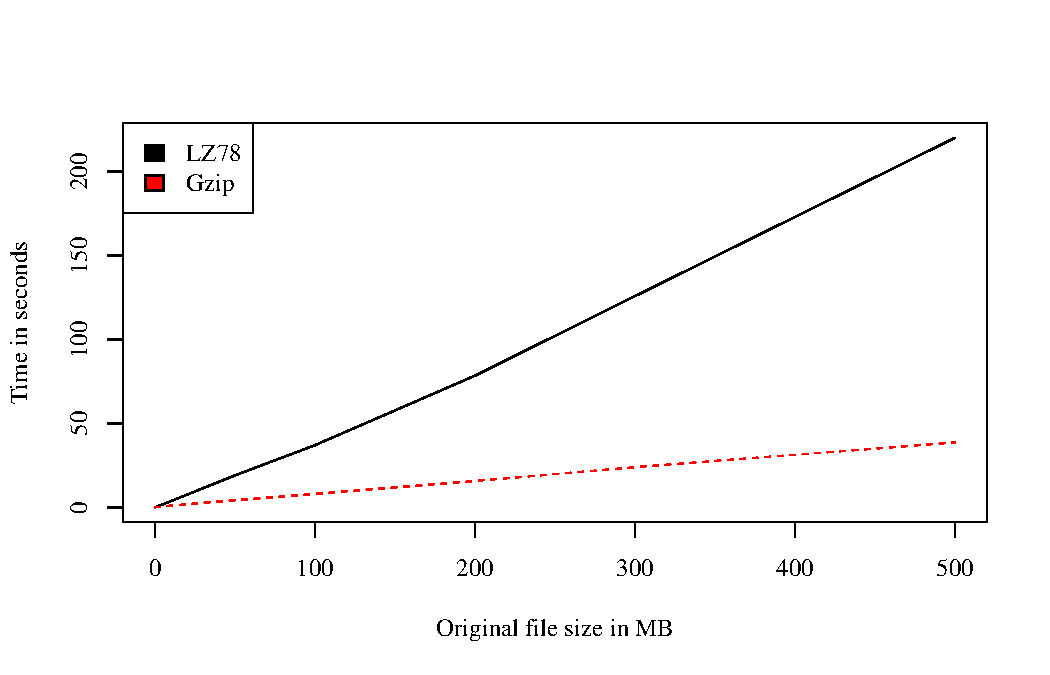
\includegraphics[scale=0.74]{../experiments/R/pdf/time_comp}
\caption{Compressão: Arquivos contendo textos em inglês}
\end{figure}

\begin{figure}
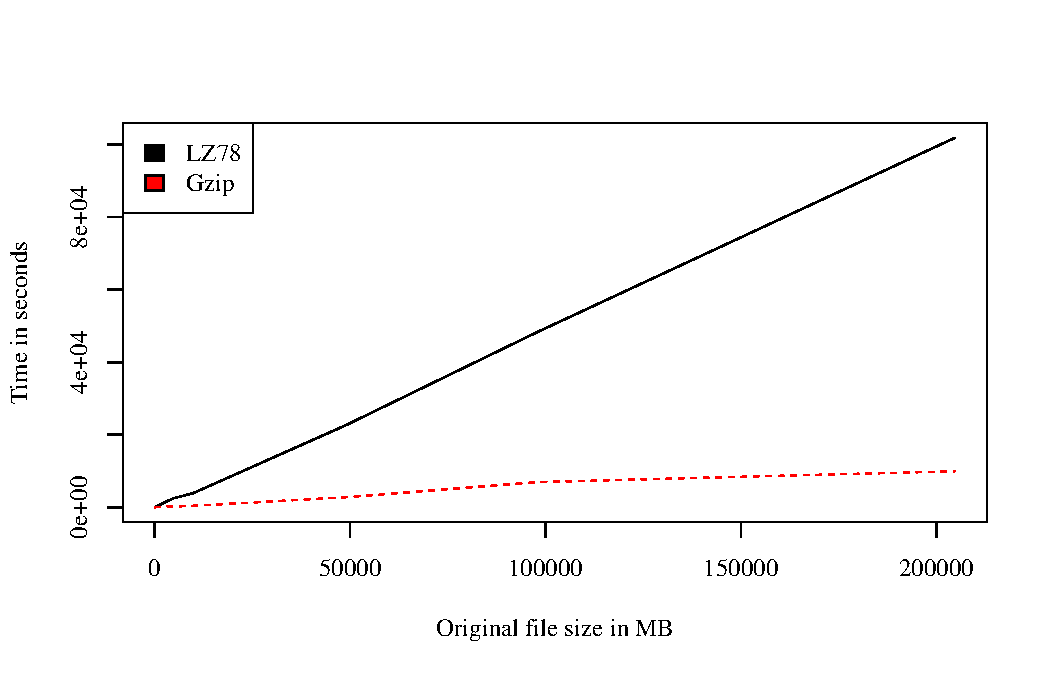
\includegraphics[scale=0.74]{../experiments/R/pdf/proteins_time_comp}
\caption{Compressão: Arquivos contendo sequência de proteinas}
\end{figure}


Abaixo estão dois gráficos que relacionam o tempo que leva para comprimir um arquivo
contendo com o tamanho dele, para ambos o nosso \lz e o \gzip. O primeiro
gráfico é referente aos arquivos contendo texto em inglês, enquanto o segundo
aos arquivos contendo sequências de proteinas.

Note que os resultados foram muito parecidos apesar do conteúdo dos arquivos
serem diferentes.
Ambas as funções de cada gráfico são (ou se aproximam muito de) retas, o que comprova que a
nossa implementação do \lz, bem como o \gzip, comprimem em tempo linear de
acordo com o tamanho do arquivo. Porém, a constante que multiplica a função do
\gzip é bem menor do que a nossa. Isso acontece porque o \gzip está em
desenvolvimento a mais de 23 anos, onde experts estão sempre otimizando o
algoritmo, fazendo com que essa constante da função linear seja cada vez menor.




Os arquivos comprimidos acima foram descomprimidos com ambas as ferramentas \lz
e \gzip.


Abaixo estão dois gráficos que relacionam o tempo que leva para descomprimir
um arquivo e o tamanho dele, um para os arquivos contendo texto em inglês e
outro para arquivos contendo sequência de proteinas.



Obtivemos novamente um resultado consistente com o anterior: ambos possuem
complexidade linear, porém a constante da descompressão do \gzip é muito
superior à da nossa implementação. Isso ficou ainda mais acentuado na
descompressão do que na compressão.

\begin{figure}[ht]
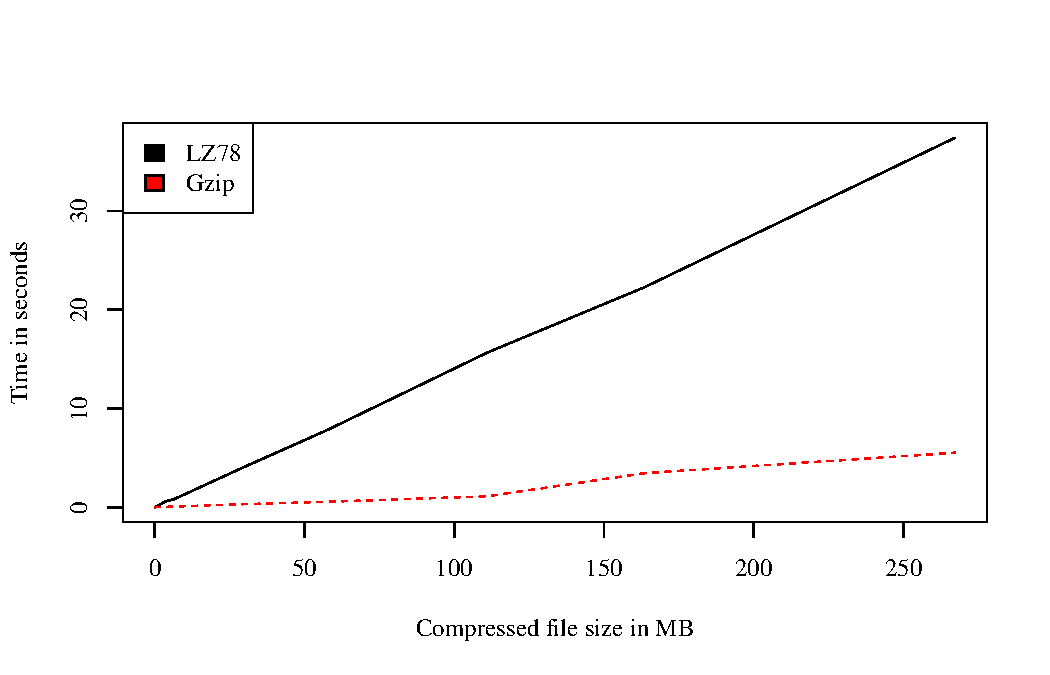
\includegraphics[scale=0.74]{../experiments/R/pdf/time_decomp}
\caption{Descompressão: Arquivos contendo textos em inglês}
\end{figure}

\begin{figure}[ht]
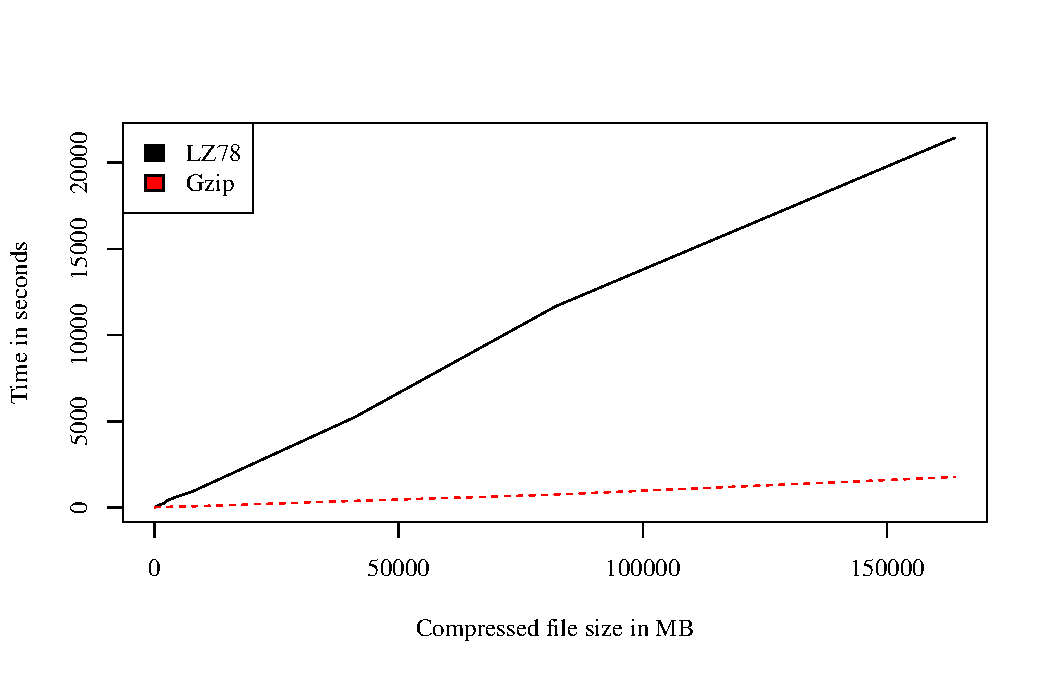
\includegraphics[scale=0.74]{../experiments/R/pdf/proteins_time_decomp}
\caption{Descompressão: Arquivos contendo sequência de proteinas}
\end{figure}



\subsubsection{Taxa de compressão}

\begin{figure}[H]
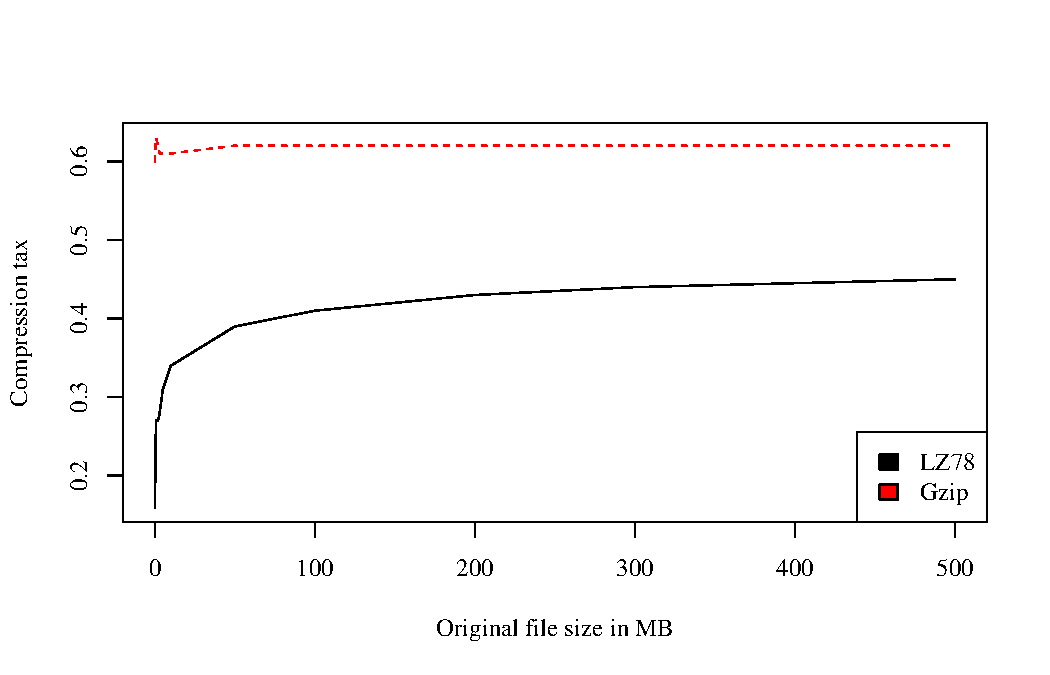
\includegraphics[scale=0.74]{../experiments/R/pdf/comp_tax}
\caption{Taxa de compressão: Arquivos contendo textos em inglês}
\end{figure}

\begin{figure}[H]
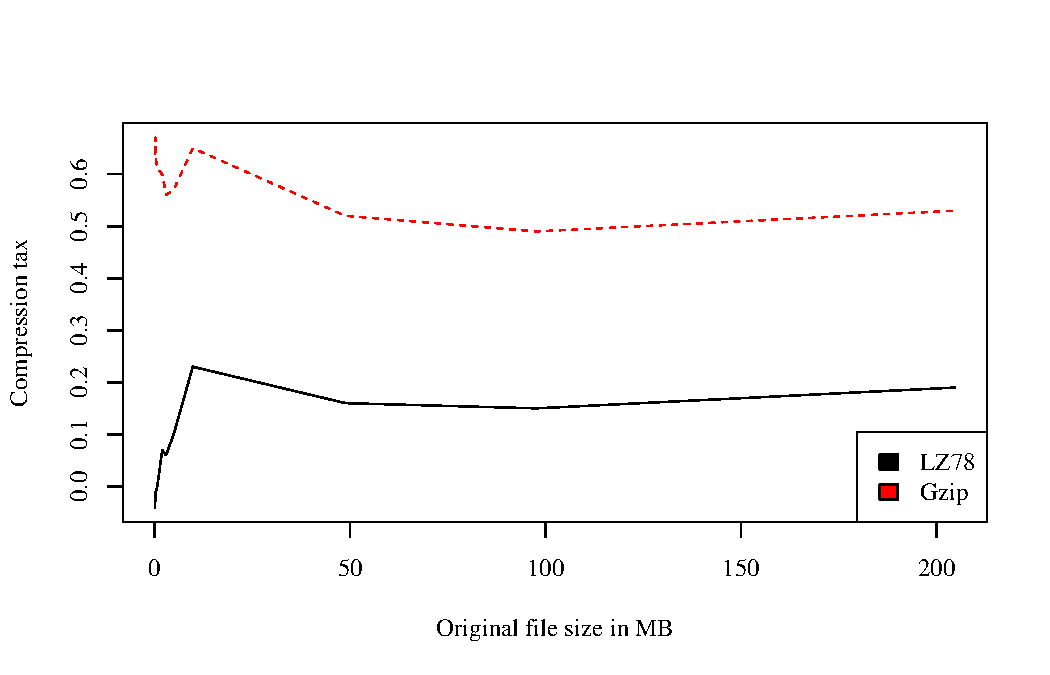
\includegraphics[scale=0.74]{../experiments/R/pdf/proteins_comp_tax}
\caption{Taxa de compressão: Arquivos contendo sequência de proteinas}
\end{figure}



Acima estão dois gráficos, um considerando arquivos de textos em inglês e outro
com arquivos contendo sequências de proteínas,
que relacionam a taxa de compressão de um arquivo com o
tamanho original dele, para ambos o nosso \lz e o \gzip.

Novamente, os resultados se assemelham quando analisados separadamente:
Ambos possuem uma variação inicial (apesar do \gzip ter uma bem menor) e se
estabilizam para arquivos maiores. Porém, para textos em inglês,
o \gzip se estabiliza com uma taxa de compressão próxima de 60\%,
enquanto que o nosso \lz se estabiliza com uma taxa
próxima de 42\%. Já para sequências de proteínas o \gzip se estabiliza com taxa
de 53\%, enquanto o \lz se estabiliza com taxa de 20\%.
Recorremos novamente ao argumento de que o \gzip está em
desenvolvimento a muito mais tempo e por isso possui mais otimizações.
Também podemos perceber que a taxa de compressão varia com o conteúdo do
arquivo, diferente da pequena diferença encontrada nos tempos de compressão e
descompessão.


\subsection{\rqtwo}
Para responder à essa pergunta nós utilizamos a ferramenta \ipmt para criar um
índice de um arquivo de texto. Após isso comparamos o tempo de realizar buscas
de diversos padrões utilizando \ipmt no arquivo indexado e comparando com o
tempo para pesquisar os padrões utilizando grep no texto original. O tempo
que leva para criar o \lsa foi desconsiderado.

Nós consideramos somente o arquivo de 50MB contendo texto inglês pelo seguinte motivo: O arquivo .idx
gerado pela ferramenta \ipmt possui ambos o texto original e o índice
comprimidos. Acontece que o array do nosso LSA tem, em média, quase 10 vezes o
tamanho do arquivo original. Ou seja, indexar e comprimir um arquivo de 50MB
acaba se tornando uma tarefa de comprimir um arquivo de aproximadamente 500MB,
que dura entre 3 e 4 minutos no nosso ambiente de experimentos. Nesse caso,
nossa compressão criou um arquivo .idx de 341MB, onde as buscas serão realizadas.
Indexar arquivos maiores do que 50MB é uma tarefa factível, mas
custosa e demorada nas nossas implementações.

Geramos randomicamente 1000 padrões (frases ou palavras em inglês): 10 padrões com tamanho de cada valor
entre 1 e 100 incluso. Após isso, realizamos a medição de tempo que o grep e
que o \ipmt levaram para buscar por esses padrões no arquivo de 50MB.
Consideramos a média entre 10 execuções de cada ferramenta. O
resultado está na figura abaixo:
\\
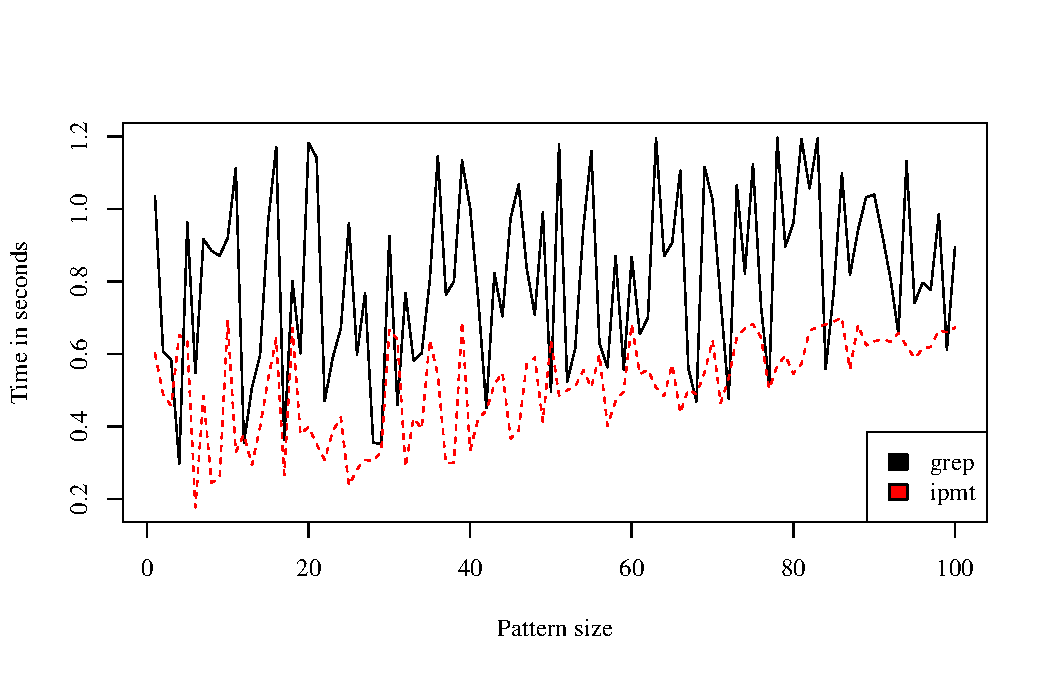
\includegraphics[scale=0.74]{../experiments/R/pdf/rq2}
\\

Podemos ver que \ipmt se saiu melhor na maioria dos casos. Isso era esperado
devido ao pré-processamento da indexação. Podemos também observar que
o tempo de resposta do grep variou independente do tamanho do padrão. Já no
\ipmt pode-se observar que quanto maior o padrão mais demorada tende a ser a
resposta. Dado que o arquivo observado foi de 50MB, para um arquivo maior do que
esse, \ipmt tende a se sair melhor ainda em relação ao grep, visto que ele varia
de acordo com o tamanho do padrão, enquanto que o grep varia de acordo com o
tamanho do texto.

\subsection{\rqthree}
Realizamos o mesmo experimento da seção anterior, porém comparando a ferramenta
\ipmt ao codesearch. Os resultados estão abaixo:
\\
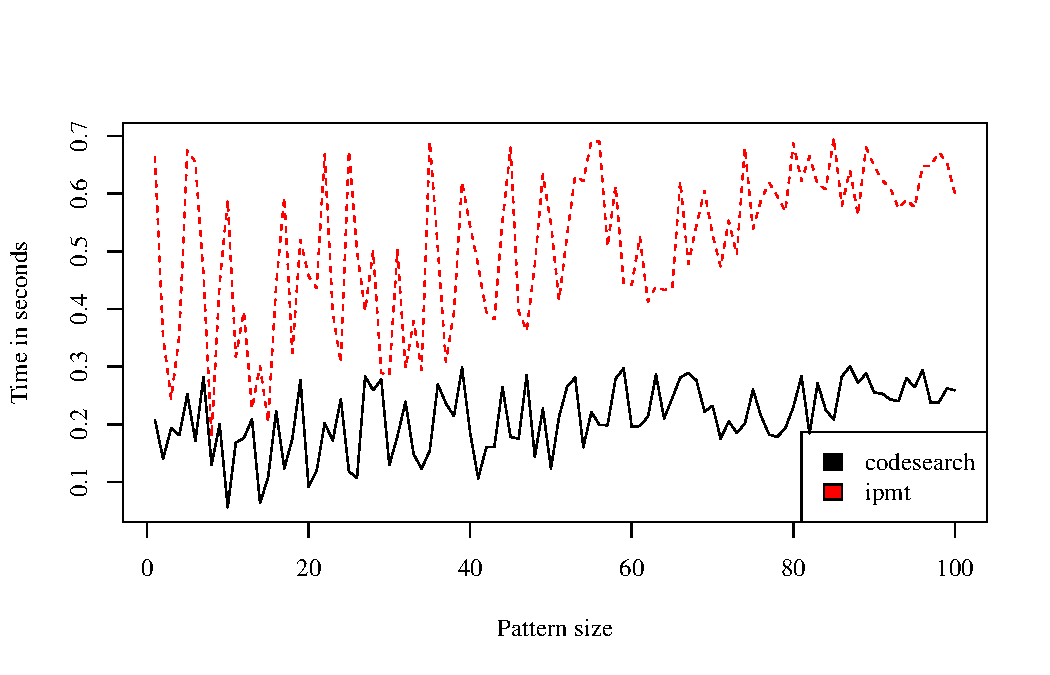
\includegraphics[scale=0.74]{../experiments/R/pdf/rq3}
\\

Visto que as médias que foram consideradas, o codesearch se saiu melhor que o
\ipmt em todos os casos.


